\documentclass{beamer}
\usetheme{Singapore}

\def\UrlBreaks{\do\/\do-} % URL breaks
\setbeamertemplate{caption}[numbered] % number figures
\setbeamertemplate{bibliography item}{\insertbiblabel} % bibliography numbers
\makeatletter
\newcommand*{\rom}[1]{\expandafter\@slowromancap\romannumeral #1@}
\makeatother

\title{Status Research Project Last-Layer Variational Inference}
\author{Philipp von Bachmann}
\institute{University of Tübingen}
\date{\today}



\begin{document}
        \begin{frame}
            \titlepage
        \end{frame}

        \begin{frame}
            \frametitle{Idea}
            \begin{itemize}
                \item Setup: Deep Learning, neural network
                \item Problem: No confidence estimates
                \item Treat the last layer of the network as bayesian
                \item Train with Variational Inference
            \end{itemize}
        \end{frame}
        
        \section{Math}
        \begin{frame}
            \frametitle{Variational Inference}
            ELBO formulation for training:
            \begin{equation}
                \log{p(y \vert x, M)} \geq \mathbb{E}_{q_{\phi}(\theta)}[\sum_{i=1}^N \log{p(y_i \vert f_{\theta}(x_i))}] - D_{KL}(q_{\phi}(\theta) \Vert p_{M}(\theta))
            \end{equation}
            $M$ model, $\theta$ network weights, $\phi$ parametrizes the variational distribution $q$ and $M$ of the prior $p$ over $\theta$
        \end{frame}

        \begin{frame}
            \frametitle{Weight distribution}
            We use a multivariate Gaussian distribution for both $q$ and $p$.
            For the covariance we have following approximations:
            \begin{itemize}
                \item mean field, corresponds to diagonal Gaussian
                \item Kronecker-Factorization
                \item Full Covariance
            \end{itemize}
        \end{frame}

        \begin{frame}
            \frametitle{Hyperparameter Tuning}
            optimize model hyperparameters $M$
            \begin{itemize}
                \item normally done by Type-\rom{2} Maximum Likelihood estimation, $p(y \vert x, M)$
                \item ELBO gives lower bound on ML $\rightarrow$ maximize
                \item alternate between normal training and hyperparameter optimization
            \end{itemize}

        \end{frame}

        \section{Examples}

        \begin{frame}
            \frametitle{Regression}
            \begin{figure}
                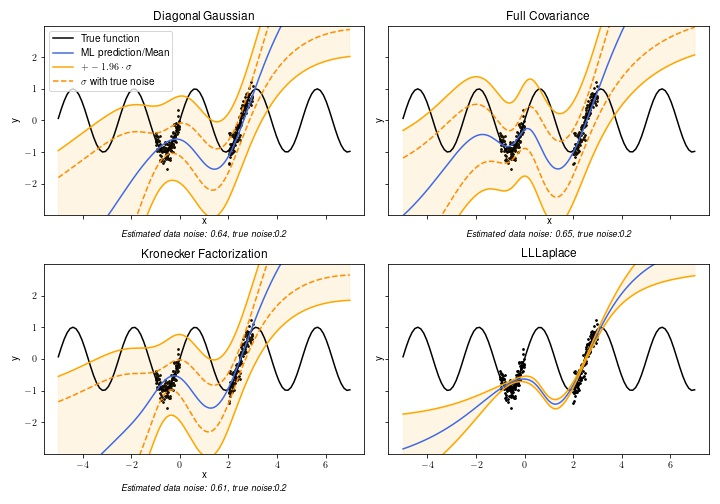
\includegraphics[width=\textwidth]{images/Regression/kernel_comparison.jpg}
            \end{figure}
        \end{frame}



        % \begin{frame}
        %     \frametitle{Regression}
        %     add regression comparison of kernels here
        %     \begin{figure}
        %         \includegraphics[width=0.8\textwidth]{images/Regression/FullCov.jpg}
        %     \end{figure}
        % \end{frame}

        % \begin{frame}
        %     \frametitle{Classification: Two Moons}
        %     add non-bayesian vs best kernel comparison here, maybe vs laplace?
        %     \begin{columns}
        %         \column{0.5\textwidth}
        %         \begin{figure}
        %             \includegraphics[width=\textwidth]{images/TowMoons/Baseline.jpg}
        %         \end{figure}
        %         \column{0.5\textwidth}
        %         \begin{figure}
        %             \includegraphics[width=\textwidth]{images/TowMoons/Diagonal.jpg}
        %         \end{figure}
        %     \end{columns}
        % \end{frame}








\end{document}
